\chapter{Introducción}

En 2010 se estimó que el consumo global de energía, para satisfacer las necesidades de 7 mil millones de personas, era de aproximadamente 13 TW (TW = 1012 W), y se pronosticó que aumentaría a 23 TW para el 2050 \cite{Kalyanasundaram}. La demanda energética se suple actualmente (en su gran mayoría) mediante combustibles fósiles, a pesar de los problemas ambientales, sociales, políticos y económicos que se han asociado a la actividad de extracción y refinamiento de petróleo, carbón, y gas natural. En este contexto, es esencial el desarrollo de fuentes de energía renovables económicamente viables. La energía solar es un buen candidato dentro de las energías renovables debido a que la radiación que llega a la Tierra proveniente del sol tiene magnitudes estimadas alrededor de 120.000 TW \cite{Kalyanasundaram} y 170.000 TW \cite{Sorensen}, y además es el flujo de entrada para todos los procesos naturales y renovables de conversión de energía del planeta, tanto biológicos como no biológicos \cite{Sorensen}. Es importante destacar también que la energía solar es limpia, segura, barata y una fuente de energía confiable sin el descargo de gases de efecto invernadero. Por estas razones, la búsqueda de tecnologías que permitan aprovechar eficientemente esta fuente de energía es un paradigma de la investigación científica a nivel global. 

Las celdas solares son los dispositivos encargados de convertir la radiación solar en energía eléctrica y se clasifican principalmente en tres clases: primera, segunda y tercera generación (ver cuadro de la figura \ref{cuadro}). Las celdas solares de \textbf{primera generación} o también llamadas celdas convencionales o tradicionales son la tecnología fotovoltaica más antigua y predominante comercialmente. Se componen de materiales de la más alta pureza con los menores defectos estructurales (como el silicio monocristalino). Las mayores eficiencias de conversión de energía obtenidas se encuentran en estas celdas, alcanzando un 26,6\%. Debido a los altos costos de mano de obra para el procesamiento del material y la importante entrada de energía requerida, el costo por W también es el más alto \cite{Yoshikawa2017,Kalyanasundaram}.
  

Como alternativa a las céldas solares de silicio, se fabrican las celdas solares de película fina o de \textbf{segunda generación} depositando una o más capas delgadas de semiconductores sobre un sustrato como vidrio, plástico o metal. Debido al alto coeficiente de absorción óptica de los semiconductores, requieren menos espesor de película. Esta tecnología siempre ha sido más barata pero menos eficiente que las celdas solares de silicio convencionales, aunque ha mejorado significativamente en la actualidad. Las principales desventajas en las celdas solares de segunda generación son el complejo proceso de deposición, la dificultad para controlar la estequiometría y la presencia de defectos estructurales \cite{C7NR08350E}. A este grupo de celdas solares de segunda generación pertenecen los paneles solares estándar comerciales.

Se han realizado varios cálculos teóricos sobre la máxima conversión de potencia obtenible mediante radiación solar. El cálculo más popular es el de Shockley-Queisser. Al considerar las celdas solares fotovoltaicas como un dispositivo con un umbral en el cuál un fotón da un electrón, estos autores estiman el 31\% como máximo bajo una iluminación solar y el 40,8\% bajo máxima luz solar concentrada. Durante la última década se han sugerido varios enfoques para reducir las pérdidas de energía y aumentar la conversión general. Los sistemas fotovoltaicos que potencialmente pueden proporcionar una eficiencia de conversión de energía por encima del límite de Shockley-Queisser están etiquetados como fotovoltaicos de \textbf{tercera generación} \cite{Kalyanasundaram}. Estas celdas se encuentran en período de investigación y tiene un costo de fabricación menor con respecto a las dos anteriores. Dentro de este grupo se encuentran las celdas solares sensibilizadas por colorantes (DSSC), celdas solares orgánicas (OSC), celdas solares de perovskita (PSC), celdas solares de punto cuántico (QDSC). 

Según el límite de Shockley-Queisser, la eficiencia teórica de una celda solar surge debido a la diferencia de energía entre la banda prohibida (o GAP) del semiconductor (SC) en la celda y el fotón solar, donde el único mecanismo de pérdida es la recombinación radiativa en la celda solar. Cualquier fotón que tenga una energía correspondiente o mayor que el GAP puede causar fotoexcitación, pero cualquier energía por debajo se pierde. El GAP del silicio es $1.1$ eV, aproximadamente la energía de la luz roja, por lo que la energía de la luz azul se pierde en una celda solar de silicio convencional. Si el GAP se sintoniza para ser mayor, digamos a la luz azul, esa energía quedará atrapada, pero solo a costa de perder fotones de menor energía \cite{Pallikkara2021}. Las celdas de tercera generación están diseñadas de tal manera que superen estos problemas, apilando capas delgadas de material con diferentes espacios entre bandas una encima de la otra, lo que se denomina enfoque de “celda en tándem” o de “unión múltiple”. Todas las celdas de tercera generación tienen un principio de funcionamiento común y se diferencian principalmente en la capa de captación de luz. Los colorantes actúan como la capa fotoactiva en las DSSC, mientras que los polímeros orgánicos conductores/moléculas orgánicas en las OSC, los compuestos con estructura de perovskita (ABX$_3$) en las PSC y los puntos cuánticos inorgánicos/orgánicos en las QDSC. Debido a algunas propiedades como el funcionamiento con poca luz y ángulos más amplios, larga vida útil, ecológicamente sano, baja toxicidad y costo de producción, técnicas de fabricación simples, etc., las DSSC son dispositivos fotovoltaicos que reciben mucha atención por parte de los investigadores. 


\forestset{
  %L1/.style={fill=green,},
  L1/.style={fill=orange,edge={orange,line width=2pt}},
  L2/.style={fill=yellow,edge={yellow,line width=2pt}},
  L3/.style={fill=pink,edge={pink,line width=2pt}},
}


\begin{figure}[h]
 \begin{forest}
  for tree={align=center}
  [Celdas Solares,L1
    [Primera Generación,L2
        [Celdas solares de Silicio,L3
        ]
    ]
    [Segunda Generación,L2
          [{Celdas solares de película fina:\\GaAs-CdTe-CIGs},L3
        ]
     ]   
    [Tercera Generación,L2
          [DSSC-OSC-\\PSC-QDSC,L3
        ]
     ]  
  ]
 \end{forest}
\caption{Clasificación de las celdas solares} 
\label{cuadro}
\end{figure}


La primera DSSC fue presentada en 1991 por O'Regan y Gr\"atzel (celda de Gr\"atzel) como un dispositivo compuesto por una película ópticamente transparente de partículas de TiO$_2$ de unos pocos nanómetros de tamaño recubierta con una monocapa de colorante para sensibilizar y recolectar de luz \cite{ORegan1991}. Los diseños iniciales de estas celdas empleaban colorantes basados en complejos de rutenio, pero hoy en dı́a existen muchos tipos de colorantes que proveen eficiencias superiores \cite{Mathew2014}. Desde el punto de vista de las posibilidades de diseño, el variar las caracterı́sticas de  los colorantes que efectúan la captura de fotones permite una gran flexibilidad en forma, color y transparencia, dando lugar a nuevas oportunidades comerciales, con la perspectiva de una inversión y fabricación a bajo costo. Esta flexibilidad significa también una mayor complejidad dado el vasto horizonte de compuestos utilizables que debe ser explorado y mapeado cuidadosamente para encontrar compuestos que brinden la mayor eficiencia posible en distintas circunstancias de iluminación, temperatura de operación, electrolito, etc. 


\begin{figure}[!htb]
 \centering
 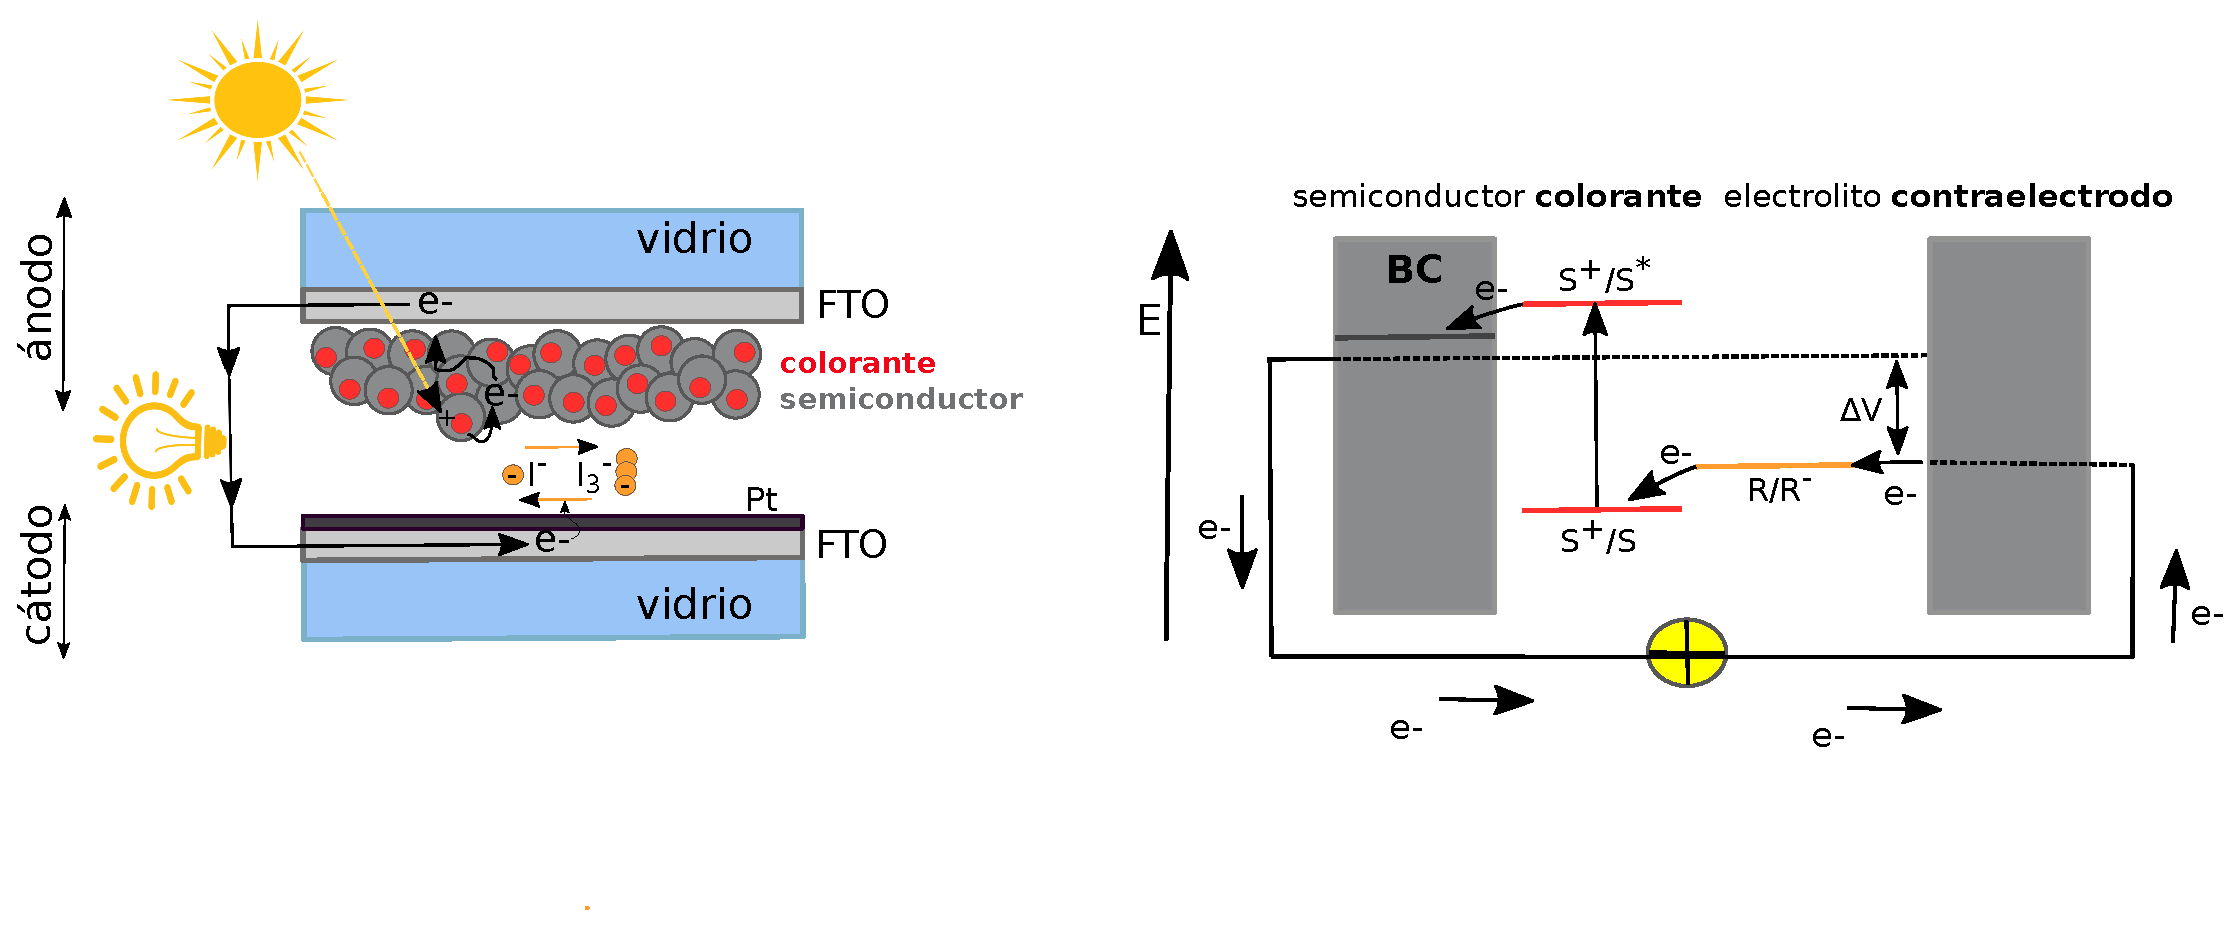
\includegraphics[height=6cm]{cap1/figs/dssc.eps}
 \caption{\textbf{(Izquierda)} esquema de una celda de Gr\"atzel y \textbf{(derecha)} representación esquemática de los principios de una celda fotovoltaica sensibilizada por colorantes indicando el nivel de energía de los electrones en las diferentes fases.}
 \label{dssc}
\end{figure}


Una DSSC está compuesta por un/a (ver figura \ref{dssc} a la izquierda): \textbf{(a)} sustrato de vidrio transparente con un óxido conductor, eventualmente óxido de estaño dopado con fluoruros (FTO), \textbf{(b)} fotoánodo, es decir, un electrodo semiconductor de óxido metálico sensibilizado por un colorante, \textbf{(c)} sustrato de vidrio con el contraelectrodo, normalmente de platino o plata que funciona como un catalizador y \textbf{(d)} solución de electrolito ubicada entre los dos electrodos.

La irradiación solar promueve la fotoexcitación del colorante y la posterior inyección de electrones desde el LUMO (de sus siglas en inglés Highest Occupied Molecular Orbital) del colorante a la banda de conduccion (BC) del SC. Al mismo tiempo, el electrolito mediante una reacción redox regenera el estado fundamental del colorante, que a su vez es regenerado por el contraelectrodo. El cierre del circuito genera una corriente cuyo voltaje máximo corresponde a la diferencia entre el nivel de fermi del SC y el potencial redox del electrolito. El funcionamiento de una DSSC se muestra en la figura \ref{dssc} a la derecha.

Existen procesos competitivos que disminuyen la fotocorriente y el fotovoltaje máximos generados en la celda:

\begin{itemize}
 \item Desactivación del estado excitado del colorante al estado fundamental.
 \item Recombinación de carga del electrón inyectado con la especie oxidada del colorante.
 \item Recombinación de carga del electrón inyectado con el electrolito.
\end{itemize}

Los niveles de energía de cada componente así como los tiempos de vida de cada una de las reacciones cinéticas que se producen, son fundamentales para el diseño de nuevos colorantes que actúen como sensibilizadores. 

En esta tesis se estudiaron los procesos que ocurren en la interfase semiconductor/colorante/electrolito de una DSSC cuando la luz del sol es captada, utilizando simulaciones computacionales como herramienta. Los capítulos 3, 4 y 5, se enfocan en el fotoelectrodo, es decir, en las interacciones entre el SC y el colorante, mientras que el capítulo 6, en las interacciones del SC con un solvente acuoso, ya que a pesar de que el agua sea un componente que está siempre presente en forma de traza y por ende en muchos casos se la considere un contaminante, científicos han considerado la posibilidad de fabricar DSSC con electrolitos a base de agua \cite{Bella2015}.

En el marco de las DSSC es fundamental que los métodos computacionales utilizados sean capaces de predecir el comportamiento de sistemas cuando se encuentran en presencia de campos externos dependientes del tiempo (sistemas fuera del equilibrio). La teorı́a del funcional de la densidad electrónica dependiente del tiempo y otros métodos basados en funciones de onda han demostrado ser una herramienta muy poderosa para estos cálculos, sin embargo, son computacionalmente costosos, pudiendo aplicarse sólo a moléculas relativamente pequeñas. El método tight-binding derivado de la teorı́a del funcional de la densidad electrónica, es el que se utiliza en esta tesis para realizar estos cálculos, y la principal ventaja es su bajo costo computacional, lo cual otorga la posibilidad de describir sistemas compuestos por miles de átomos. Es un método alternativo para estudiar la dinámica cuántica en tiempo real basado en la propagación de la matriz densidad reducida de un electrón. 

\section{Objetivos}

\subsection{Objetivo General}

El objetivo general del presente proyecto es comprender los mecanismos dinámicos en los que se fundamenta la captación de energı́a en sistemas nanoestructurados sensibilizados con colorantes dentro y fuera del régimen de respuesta lineal.

El objetivo general del presente proyecto es comprender las propiedades ópticas (dentro y fuera del régimen de respuesta lineal) y catalíticas de sistemas nanoestructurados.

\subsection{Objetivos específicos}

\begin{itemize}
 \item Desarrollar un modelo simple para la transferencia de carga fotoinducida en sistemas colorante-nanopartı́cula.
 \item Describir el espacio de parámetros del modelo y validarlo comparando con resultados obtenidos a partir de simulaciones de dinámica cuántica.
 \item Estudiar las propiedades ópticas de nanopartículas de TiO$_2$ sensibilizadas con colorantes al iluminar con radiación de banda ancha. 
 \item Estudiar las propiedades ópticas de nanowires de ZnO con distintos cubrimientos de catecol.
 \item Estudiar los efectos del agua y el desorden térmico en nanowires de ZnO.
 \item Validar estructuralmente, termodinámicamente y cinéticamente el potencial ReaxFF y dftb+ con respecto a DFT en sistemas ZnO-agua.
\end{itemize}
